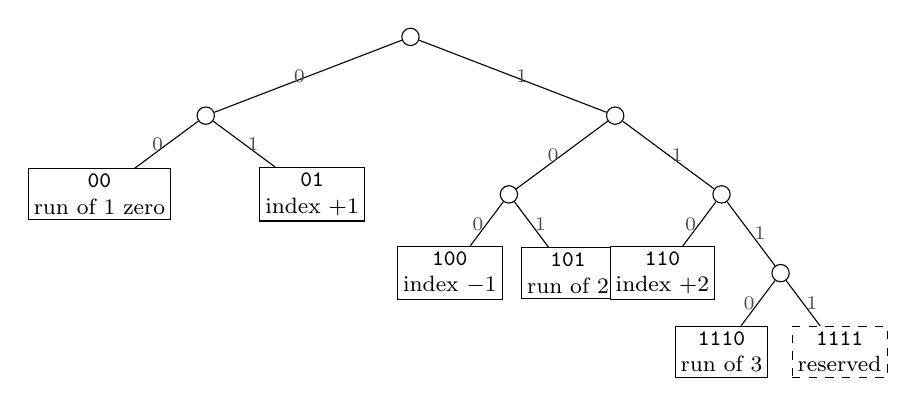
\begin{tikzpicture}[level distance=10mm,font=\footnotesize,
    inner/.style={circle,draw,fill=white,inner sep=0pt,minimum size=2.2mm},
    leaf/.style={draw,align=center,inner sep=2pt,fill=white},
    level 1/.style={sibling distance=52mm},
    level 2/.style={sibling distance=27mm},
    level 3/.style={sibling distance=15mm},
    edge from parent/.style={draw},
    bit/.style={font=\scriptsize,text=black!70,inner sep=1pt}]
  \node[inner] {}
    child {node[inner] {}
      child {node[leaf] {\texttt{00}\\run of 1 zero} edge from parent node[bit,left] {0}}
      child {node[leaf] {\texttt{01}\\index $+1$} edge from parent node[bit,right] {1}}
      edge from parent node[bit,left] {0}}
    child {node[inner] {}
      child {node[inner] {}
        child {node[leaf] {\texttt{100}\\index $-1$} edge from parent node[bit,left] {0}}
        child {node[leaf] {\texttt{101}\\run of 2} edge from parent node[bit,right] {1}}
        edge from parent node[bit,left] {0}}
      child {node[inner] {}
        child {node[leaf] {\texttt{110}\\index $+2$} edge from parent node[bit,left] {0}}
        child {node[inner] {}
          child {node[leaf] {\texttt{1110}\\run of 3} edge from parent node[bit,left] {0}}
          child {node[leaf,dashed] {\texttt{1111}\\reserved} edge from parent node[bit,right] {1}}
          edge from parent node[bit,right] {1}}
        edge from parent node[bit,right] {1}}
      edge from parent node[bit,right] {1}};
\end{tikzpicture}
